
% Theory part goes here %

% for numerated formulas
\newcommand{\formula}[3]
{
    \noindent#1\\[0.1cm]
    \begin{equation}\label{#2}
        #3
    \end{equation}
}

% for in-text math formulas
\newcommand{\mth}[1]
{
    \begin{math}
        #1
    \end{math}
}

% for rus letters in indexes
\newcommand{\ruB}[1]
{
    _{\text{#1}}
}

\section{Теория}

\subsection {Схема установки}

Схема установки представлена на рисунке 1.

\begin{center}

    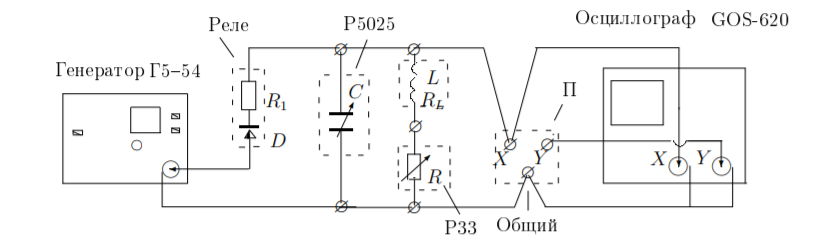
\includegraphics[scale=0.9]{324-scheme.png} \\
    \textit{Рис. 1. Схема установки}

\end{center}

\subsection {Исследуемые величины}

В работе планируется:

\begin{enumerate}
    \item Исследовать зависимость периода свободных колебаний контура от емкости. Согласно теории, зависимость должна иметь вид (Формула Томпсона):

    \formula
    {}
    {Tompson}
    {T = 2\pi \sqrt{LC} \quad,}

    где T - период колебаний, L и C - индуктивность и емкость контура соответственно.

    Период планируется измерять с помощью осциллографа.

    \item Исследовать зависимость логарифмического декремента затухания от сопротивления. \\ Расчет логарифмического декремента затухания будет производиться по следующей формуле:

    \formula
    {}
    {Decrement}
    {\lambda = \frac{1}{n} \ln\frac{W_k}{W_{k+n}} \quad,}

    где \mth{W_i} - энергия контура после i-того колебания.

    Энергию контура планируется высчитывать используя напряжение на конденсаторе, которое в свою очередь, измеряется с помощью осциллографа. \\

    \formula
    {Согласно теории, логарифмический декремент затухания пропорционалени сопротивлению}
    {DecrPropR}
    {\lambda \propto R}

    \newpage

    \item Определить критическое сопротивление. Критическое сопротивление вычисляется по формуле:

    \formula
    {}
    {CriticalR}
    {R\ruB{кр} = 2\sqrt{\frac{L}{C}}}

    \item Определить добротность контура. Добротность планируется вычислить двумя способами, с последующим сравнением результатов. \\

    Первый способ - Через формулу для логарифмического декремента затухания. \\
    Второй способ - используя параметры контура R, L, C. \\[0.1cm]

    \formula
    {Формула для вычисления добротности через логарифмический декремент затухания:}
    {qualityFactorFt}
    {Q = \frac{\pi}{\lambda}}

    \formula
    {Формула для вычисления добротности с использованием параметров контура}
    {qualityFactorSd}
    {Q = \frac{1}{R} \sqrt{\frac{L}{C}}}

\end{enumerate}

\subsection {Методы проверки зависимостей}

Для проверки теоретических зависимостей проще всего сводить эти зависимости к линейным уравнениям исследуемых величин (тогда графики будут наглядными и отклонения от нормы будут более заметны). \\

\noindent В связи с этим будут построены графики зависимостей (\ref{linearT}) и (\ref{linearLmbd}):

\formula
{}
{linearT}
{T^2 (LC) \quad,}
\formula
{тогда зависимость, согласно теории, будет иметь линейный вид:}
{linearTEquation}
{T^2 = 4\pi^2LC}

\formula
{}
{linearLmbd}
{\lambda(R) \quad,}
здесь зависимость и так линейная